\documentclass[11pt,a4paper]{article}

\usepackage[a4paper,margin=23mm]{geometry}
\usepackage{amsmath,amssymb,mathtools}
\usepackage{physics}
\usepackage{siunitx}
\usepackage{microtype}
\usepackage{booktabs}
\usepackage{array}
\usepackage{enumitem}
\usepackage[dvipsnames]{xcolor}
\usepackage[most]{tcolorbox}
\usepackage{tikz}
\usepackage{pgfplots}
\usepackage{hyperref}
\usepackage{fancyhdr}
\usepackage{titlesec}
\usepackage{tocloft}
\usepackage{setspace}
\usepackage{lastpage}
\setlength{\headheight}{14pt}

\pgfplotsset{compat=1.18}
\usetikzlibrary{arrows.meta,calc,decorations.pathreplacing,positioning,angles,quotes}

\definecolor{DeepBlue}{HTML}{1F4E79}
\definecolor{SoftBlue}{HTML}{EAF3FA}
\definecolor{DeepGreen}{HTML}{2F6B45}
\definecolor{SoftGreen}{HTML}{EDF7ED}
\definecolor{WarmOrange}{HTML}{C56A1A}
\definecolor{SoftOrange}{HTML}{FFF3E6}
\definecolor{DeepRed}{HTML}{8A1C1C}
\definecolor{SoftRed}{HTML}{FDECEC}
\definecolor{GraphGrey}{HTML}{5C6670}

\hypersetup{
    colorlinks=true,
    linkcolor=DeepBlue,
    urlcolor=DeepBlue,
    citecolor=DeepBlue,
    pdftitle={From Situation to Formula: Projectile Motion as a Language of Physics},
    pdfauthor={Prepared lecture notes},
    pdfsubject={Physics Basics},
    pdfkeywords={physics, mathematics, projectile motion, modelling, interpretation}
}

\setstretch{1.08}
\setlength{\parindent}{0pt}
\setlength{\parskip}{0.62em}
\setlist[itemize]{topsep=0.35em,itemsep=0.2em,leftmargin=1.5em}
\setlist[enumerate]{topsep=0.35em,itemsep=0.25em,leftmargin=1.8em}

\pagestyle{fancy}
\fancyhf{}
\lhead{From Situation to Formula}
\rhead{Projectile Motion}
\cfoot{\thepage\ / \pageref{LastPage}}

\titleformat{\section}{\Large\bfseries\color{DeepBlue}}{\thesection}{0.75em}{}
\titleformat{\subsection}{\large\bfseries\color{DeepGreen}}{\thesubsection}{0.75em}{}
\titleformat{\subsubsection}{\normalsize\bfseries\color{WarmOrange}}{\thesubsubsection}{0.75em}{}

\newtcolorbox{principlebox}[1]{
  enhanced, breakable,
  colback=SoftBlue, colframe=DeepBlue,
  arc=2mm, boxrule=0.8pt,
  left=2mm,right=2mm,top=1.2mm,bottom=1.2mm,
  title={#1}, fonttitle=\bfseries
}

\newtcolorbox{methodbox}[1]{
  enhanced, breakable,
  colback=SoftGreen, colframe=DeepGreen,
  arc=2mm, boxrule=0.8pt,
  left=2mm,right=2mm,top=1.2mm,bottom=1.2mm,
  title={#1}, fonttitle=\bfseries
}

\newtcolorbox{warningbox}[1]{
  enhanced, breakable,
  colback=SoftOrange, colframe=WarmOrange,
  arc=2mm, boxrule=0.8pt,
  left=2mm,right=2mm,top=1.2mm,bottom=1.2mm,
  title={#1}, fonttitle=\bfseries
}

\newtcolorbox{examplebox}[1]{
  enhanced, breakable,
  colback=white, colframe=GraphGrey,
  arc=2mm, boxrule=0.55pt,
  left=2mm,right=2mm,top=1.2mm,bottom=1.2mm,
  title={#1}, fonttitle=\bfseries\color{black}
}

\newcommand{\g}{g}
\newcommand{\vzero}{v_0}
\newcommand{\vx}{v_{0x}}
\newcommand{\vy}{v_{0y}}
\newcommand{\x}{x}
\newcommand{\y}{y}
\newcommand{\tflight}{t_{\mathrm{flight}}}
\newcommand{\tup}{t_{\mathrm{up}}}
\newcommand{\R}{R}
\newcommand{\Hmax}{H_{\max}}
\newcommand{\vect}[1]{\boldsymbol{#1}}

\begin{document}

\begin{titlepage}
\centering
\vspace*{18mm}
{\Huge\bfseries\color{DeepBlue} From Situation to Formula\\[2mm]}
{\LARGE\bfseries Projectile Motion as a Language of Physics\\[8mm]}
{\Large Lecture recap notes for Physics Basics\\[15mm]}
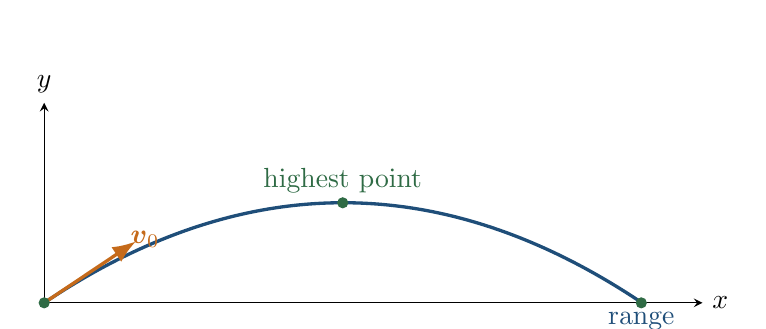
\begin{tikzpicture}[scale=1.0]
  \begin{axis}[
    width=0.82\textwidth,height=0.34\textwidth,
    axis lines=left,
    xmin=0,xmax=86,ymin=0,ymax=32,
    xlabel={$x$},ylabel={$y$},
    xtick=\empty, ytick=\empty,
    clip=false,
    every axis x label/.style={at={(current axis.right of origin)},anchor=west},
    every axis y label/.style={at={(current axis.above origin)},anchor=south}
  ]
  \addplot[DeepBlue, very thick, domain=0:78, samples=150] {0.82*x - 0.0105*x*x};
  \addplot[mark=*, only marks, mark size=1.8pt, DeepGreen] coordinates {(0,0) (78,0) (39,16)};
  \node[DeepGreen, anchor=south] at (axis cs:39,16) {highest point};
  \node[DeepBlue, anchor=north] at (axis cs:78,0) {range};
  \draw[-{Latex[length=3mm]}, WarmOrange, very thick] (axis cs:0,0) -- (axis cs:12,9.84);
  \node[WarmOrange, anchor=west] at (axis cs:10,10.2) {$\vect v_0$};
  \end{axis}
\end{tikzpicture}
\vfill
{\large A document about how physics uses mathematics: not as a pile of formulas, but as a compact language for relations, questions, transformations, and interpretations.}
\vfill
{\large \today}
\end{titlepage}

\tableofcontents
\newpage

\section*{How to use these notes}
\addcontentsline{toc}{section}{How to use these notes}

These notes are meant for a recap lecture in which projectile motion is not treated as one more exercise in substituting numbers into a known formula. The goal is more fundamental: to show how a physical situation is translated into mathematical language, how mathematical work is performed inside that language, and how the result is translated back into physical meaning.

The central example is deliberately simple: a point-like object is launched, gravity acts downward, air resistance is ignored. This model is not chosen because the world is always that simple. It is chosen because the mathematical structure is visible. In one example we can see vectors, components, functions, derivatives, integrals, equations, roots, maxima, parameters, constraints, and interpretation.

\begin{principlebox}{Main message}
A formula is not the beginning of physics. A formula is a compressed record of assumptions, definitions, relations, and questions. Before we use a formula, we must know what situation it describes, what it ignores, what each symbol means, and what question we are asking.
\end{principlebox}

The document is written as a narrative rather than as a list of final results. Each important calculation is placed inside the same loop:
\[
\begin{aligned}
&\text{physical situation}\quad\longrightarrow\quad\text{mathematical model}\\
&\longrightarrow\quad\text{mathematical work}\quad\longrightarrow\quad\text{physical interpretation}.
\end{aligned}
\]

That loop is the real topic of the lecture.

\newpage

\section{The problem with treating physics as a list of formulas}

Many students say: ``Which formula should I use?'' This question is understandable, but it is often the wrong first question. It assumes that physics is a catalogue of equations and that solving a problem means recognizing the correct equation, inserting numbers, and simplifying.

There are situations where this works mechanically. If a problem says ``use Ohm's law'', gives $U$ and $R$, and asks for $I$, then the calculation is short. But this is not the structure of physics. Physics does not begin with a formula. It begins with a situation in the world, a question about that situation, and a decision about what aspects of the situation are essential.

A formula such as
\[
F = ma
\]
is not merely an instruction to multiply two numbers. It states a relation between force, mass, and acceleration inside a particular theoretical framework. It also hides a definition of acceleration, a choice of inertial reference frame, and an assumption that the mass is constant in the usual elementary setting. If the acceleration changes with time, the formula still makes sense, but now it becomes a statement about functions:
\[
F(t) = m a(t).
\]
If motion is two-dimensional, it becomes a vector relation:
\[
\vect F(t) = m\vect a(t).
\]
The symbol $F$ is therefore not just a box where we put a number. It may represent a scalar magnitude, a component, or a vector, depending on how the model is set up.

\begin{warningbox}{A common false picture}
False picture: physics problem $=$ choose formula $+$ substitute numbers.\\
Better picture: physics problem $=$ understand the situation $+$ choose variables $+$ write relations $+$ ask a mathematical question $+$ interpret the result.
\end{warningbox}

The word ``formula'' often hides a lack of distinction between several different things:
\begin{itemize}
    \item a definition, for example $v=\dv{x}{t}$;
    \item a law of nature or a model law, for example $\vect F=m\vect a$;
    \item a derived consequence, for example $y(x)=x\tan\theta-\dfrac{g x^2}{2v_0^2\cos^2\theta}$;
    \item a special-case shortcut, for example $R=\dfrac{v_0^2\sin(2\theta)}{g}$;
    \item a condition answering a question, for example $y(t)=0$ for landing on the ground.
\end{itemize}

When all of these are called simply ``formulas'', the structure disappears. Then students try to memorize final expressions without understanding what questions produced them. In these notes we will do the opposite: we will begin with questions and watch formulas appear as compressed answers.

\section{What equations actually do}

An equation is a sentence written in mathematical grammar. It may say that two quantities are equal, that a certain object has a certain property, or that a relation must hold under certain conditions. The equation
\[
y(t)=y_0+v_{0y}t-\frac{1}{2}gt^2
\]
is a sentence about vertical position as a function of time. It says: start at height $y_0$, begin with vertical velocity $v_{0y}$, and change vertical velocity at a constant rate $-g$. The square in $t^2$ is not decorative. It is the mathematical fingerprint of constant acceleration.

A different equation,
\[
y(t)=0,
\]
is not a law of motion. It is a condition. It says: find the time when the projectile is at ground level. The expression for $y(t)$ describes the whole vertical motion; the equation $y(t)=0$ selects particular moments from that motion.

A third equation,
\[
\dv{y}{t}=0,
\]
is also not the same kind of object. It is a condition for a horizontal tangent in the graph of $y(t)$, which in projectile motion corresponds to the highest point. It says: at the top, the vertical velocity is zero.

\begin{principlebox}{One expression, many questions}
The expression $y(t)=y_0+v_{0y}t-\frac12gt^2$ is not one problem. It is a model from which many questions can be asked: When is $y=0$? When is $y$ maximal? What is the height after two seconds? How does the answer change when $v_{0y}$ changes? Each question becomes a different mathematical operation.
\end{principlebox}

This is why the same mathematical object can appear in many tasks. Students often think that a new question requires a new formula. Very often it does not. A new question requires a new interpretation of the same model.

\section{The translation loop}

The most important skill in elementary physics is not algebra alone. It is translation. We translate ordinary language into mathematical language, perform mathematical operations, and translate back.

Consider the sentence:

\emph{The projectile hits the ground.}

In the model, the ground is represented by the horizontal line $y=0$. The sentence therefore becomes
\[
y(t)=0.
\]
This equation does not immediately give a number. It gives a mathematical task: solve a quadratic equation for $t$. The positive solution is then interpreted as the time of flight.

Consider another sentence:

\emph{The projectile reaches its highest point.}

The highest point is not defined by a special label attached to the projectile. It is defined by a maximum of the height function. Mathematically, we can express it by
\[
\dv{y}{t}=0
\]
or, when viewing the trajectory as a graph $y(x)$, by
\[
\dv{y}{x}=0.
\]
The two approaches describe the same physical point, but they organize the problem differently.

\begin{methodbox}{The modelling loop}
For every problem, ask four questions in this order:
\begin{enumerate}
    \item What physical situation is being described?
    \item What quantities and assumptions define the model?
    \item What mathematical condition represents the question?
    \item What does the mathematical answer mean physically?
\end{enumerate}
\end{methodbox}

The loop is more important than any single final expression. If a student understands the loop, the number of formulas to memorize decreases drastically.

\section{Minimal mathematical language needed for the lecture}

Projectile motion is a small physical model, but it uses a surprisingly rich mathematical vocabulary. We need only a few tools, but we need to understand what each tool means.

\subsection{Variables and parameters}

A variable changes inside the problem. A parameter is fixed while we analyze the problem, but can be changed between different versions of the problem. For example, in
\[
y(t)=y_0+v_{0y}t-\frac12gt^2,
\]
the variable is $t$. The quantities $y_0$, $v_{0y}$, and $g$ are parameters for one particular launch. If we ask how the range changes when the angle changes, then the angle $\theta$ becomes the variable of a new function $R(\theta)$.

This distinction is essential. The same letter can have different roles in different stages of the analysis. In one question, $\theta$ is fixed and $t$ changes. In another question, the time of flight has already been eliminated and $\theta$ becomes the quantity we vary to optimize range.

\subsection{Functions}

A function is not just a formula. A function describes dependence. The notation
\[
y(t)
\]
means that the vertical coordinate is being considered as a quantity depending on time. The notation
\[
y(x)
\]
means that the vertical coordinate is being considered as a quantity depending on the horizontal coordinate. These are not the same viewpoint.

The projectile has one motion, but we can describe it in several mathematical languages:
\begin{align*}
\text{time description:} && x(t),\quad y(t), \\
\text{trajectory description:} && y(x), \\
\text{range as angle function:} && R(\theta), \\
\text{height as parameter function:} && H_{\max}(v_0,\theta).
\end{align*}
Each form is useful for a different kind of question.

\subsection{Derivatives}

A derivative measures rate of change. In motion, derivatives connect position, velocity, and acceleration:
\[
\vect v(t)=\dv{\vect r}{t}, \qquad \vect a(t)=\dv{\vect v}{t}=\dv[2]{\vect r}{t}.
\]
This is not a decorative chain of symbols. It encodes the idea that velocity tells us how position changes, and acceleration tells us how velocity changes.

When we say that the projectile is at its highest point, we mean that the height is temporarily not increasing and not yet decreasing. In mathematical language, the derivative of height with respect to time is zero:
\[
\dv{y}{t}=0.
\]
That derivative is exactly the vertical component of velocity. So the mathematical condition is also the physical statement
\[
v_y=0.
\]

\subsection{Integrals}

If derivatives move from position to velocity to acceleration, integrals move in the opposite direction. If acceleration is known, integrating gives velocity; integrating velocity gives position:
\[
a_y=-g \quad\Longrightarrow\quad v_y(t)=v_{0y}-gt
\]
and
\[
v_y(t)=v_{0y}-gt \quad\Longrightarrow\quad y(t)=y_0+v_{0y}t-\frac12gt^2.
\]
The constant of integration is not an abstract inconvenience. It is the initial condition. Physics enters the mathematical solution through these constants.

\subsection{Equations and inequalities}

When we solve
\[
y(t)=0,
\]
we find exact moments at which the projectile is at ground level. When we write
\[
y(t)>0,
\]
we describe the time interval during which the projectile is above ground. When we write
\[
y_1<y(t)<y_2,
\]
we describe the projectile passing through a vertical window. Equations locate boundaries; inequalities describe regions.

This distinction matters because physical questions are not always of the form ``find the value''. Sometimes the question is ``during what interval'', ``under what conditions'', or ``is it possible''. Mathematical language can express all of these.

\newpage

\section{The physical scene: one launch, many possible questions}

Imagine that a small object is launched from a point. It leaves the hand, a cannon, or a device with an initial speed $v_0$ at an angle $\theta$ above the horizontal. After launch we ignore air resistance. The only force is gravity, directed downward.

This is a model, not a photograph of reality. Real balls have size, spin, drag, turbulence, deformation, and contact effects. The purpose of the model is to isolate one structure: motion with constant downward acceleration.

\begin{center}
\begin{tikzpicture}[scale=1.05]
\draw[->, thick] (0,0) -- (9,0) node[right] {$x$};
\draw[->, thick] (0,0) -- (0,4.8) node[above] {$y$};
\draw[DeepBlue, very thick, domain=0:8.2, samples=100] plot (\x,{0.85*\x-0.1*\x*\x});
\draw[-{Latex[length=3mm]}, WarmOrange, very thick] (0,0) -- (1.5,1.275) node[above right] {$\vect v_0$};
\draw[dashed, GraphGrey] (1.5,0) -- (1.5,1.275);
\draw[dashed, GraphGrey] (0,1.275) -- (1.5,1.275);
\draw[-{Latex[length=2.5mm]}, DeepGreen, thick] (0.2,4.2) -- (0.2,3.2) node[midway,right] {$\vect g$};
\draw (0.75,0) arc[start angle=0,end angle=40.36,radius=0.75];
\node at (0.95,0.28) {$\theta$};
\fill[DeepGreen] (0,0) circle (2pt) node[below left] {launch};
\fill[DeepGreen] (8.2,0) circle (2pt) node[below] {landing};
\end{tikzpicture}
\end{center}

From this single scene we can ask many different questions:
\begin{itemize}
    \item Where is the projectile after a given time?
    \item How long is it in the air?
    \item How far does it travel horizontally before landing?
    \item What is the maximum height?
    \item At what time does it reach the maximum height?
    \item What launch angle gives the greatest range?
    \item Can the projectile hit a specified target?
    \item Will it pass through a specified window?
    \item How do the answers change when the initial speed changes?
\end{itemize}

The remarkable point is that we do not need a separate physical law for each question. We need one model, and then we ask different mathematical questions inside that model.

\section{Choosing coordinates is part of the model}

Before writing equations, we choose coordinates. This choice is not forced by nature. It is our decision. A good coordinate system makes the problem easier to express.

For projectile motion near Earth's surface, we usually choose:
\begin{itemize}
    \item the $x$-axis horizontal,
    \item the $y$-axis vertical upward,
    \item the origin at the launch point or at ground level below the launch point,
    \item time $t=0$ at the instant of launch.
\end{itemize}

With this convention, gravity points in the negative $y$ direction. Therefore the acceleration vector is
\[
\vect a=(0,-g).
\]
The number $g$ is positive, approximately $9.81\,\mathrm{m/s^2}$ near Earth's surface. The minus sign is not part of $g$ itself. The minus sign comes from our coordinate choice: upward is positive, gravity points downward.

\begin{warningbox}{Sign convention}
Do not say vaguely that ``gravity is negative''. Gravity has a direction. In our coordinate system, its vertical component is negative because the positive $y$ direction points upward.
\end{warningbox}

The initial velocity vector is decomposed into components:
\[
\vect v_0=(v_0\cos\theta,\,v_0\sin\theta).
\]
This expression is not a new physical law. It is trigonometry applied to the initial velocity vector. The horizontal component tells how fast the object initially moves sideways; the vertical component tells how fast it initially moves upward.

\subsection{Why components matter}

The projectile motion model becomes simple because the horizontal and vertical components behave differently:
\begin{align*}
\text{horizontal:} && a_x&=0, \\
\text{vertical:} && a_y&=-g.
\end{align*}
There is no horizontal acceleration in the ideal model, because we ignore air resistance and assume no horizontal force after launch. The vertical acceleration is constant because gravity is assumed constant.

This is the first major example of translation. The physical sentence

\emph{Only gravity acts after launch}

becomes the mathematical statement
\[
\vect a=(0,-g).
\]

\section{From force to acceleration}

The physical law behind the model is Newton's second law:
\[
\vect F=m\vect a.
\]
After launch, the only force is the weight of the object:
\[
\vect F=(0,-mg).
\]
Therefore
\[
 m\vect a=(0,-mg).
\]
Assuming $m\ne0$, divide by $m$:
\[
\vect a=(0,-g).
\]

This short derivation contains an important physical idea: in this model, the acceleration does not depend on the mass of the projectile. A heavy object and a light object have the same gravitational acceleration if air resistance is neglected.

\begin{principlebox}{Meaning of the mass cancellation}
The mass disappears not because mass is irrelevant in all of physics, but because gravitational force is proportional to mass and Newton's law also contains mass. In this model the two appearances cancel. If air resistance were included, mass would matter again.
\end{principlebox}

The result $\vect a=(0,-g)$ is the seed from which the rest of the model grows. It is not yet the trajectory. It is the rule for how velocity changes.

\section{From acceleration to velocity}

Acceleration is the derivative of velocity:
\[
\vect a(t)=\dv{\vect v}{t}.
\]
Since
\[
\vect a(t)=(0,-g),
\]
we integrate component by component.

Horizontal component:
\[
\dv{v_x}{t}=0.
\]
A function with zero derivative is constant, so
\[
v_x(t)=v_{0x}=v_0\cos\theta.
\]
The horizontal velocity does not change in this model.

Vertical component:
\[
\dv{v_y}{t}=-g.
\]
Integrating gives
\[
v_y(t)=v_{0y}-gt=v_0\sin\theta-gt.
\]
The vertical velocity decreases linearly with time. It starts positive if the object is launched upward, becomes zero at the top, and becomes negative during the fall.

\begin{methodbox}{Interpretation of the velocity equations}
\[
v_x(t)=v_0\cos\theta
\]
means constant horizontal motion.\\
\[
v_y(t)=v_0\sin\theta-gt
\]
means uniformly changing vertical motion.\\
The projectile is one object, but the coordinate description separates the motion into two simpler stories.
\end{methodbox}

\section{From velocity to position}

Velocity is the derivative of position:
\[
\vect v(t)=\dv{\vect r}{t}.
\]
Therefore we integrate once more.

Horizontal component:
\[
\dv{x}{t}=v_0\cos\theta.
\]
If the initial horizontal position is $x_0$, then
\[
x(t)=x_0+v_0\cos\theta\,t.
\]
Often we choose $x_0=0$, so
\[
x(t)=v_0\cos\theta\,t.
\]

Vertical component:
\[
\dv{y}{t}=v_0\sin\theta-gt.
\]
If the initial vertical position is $y_0$, then
\[
y(t)=y_0+v_0\sin\theta\,t-\frac12gt^2.
\]

Together:
\[
\boxed{\vect r(t)=\left(x_0+v_0\cos\theta\,t,\; y_0+v_0\sin\theta\,t-\frac12gt^2\right).}
\]

This is the parametric description of projectile motion. The parameter is time. At each time $t$, the formulas give both coordinates.

\subsection{Where the initial conditions entered}

The constants $x_0$, $y_0$, $v_0$, and $\theta$ are not arbitrary algebraic ornaments. They describe the launch. Without them, the equation would not specify a particular motion. This is why initial conditions are not secondary details. They connect the mathematical solution to the physical situation.

If we launch from the ground, we often set $x_0=0$ and $y_0=0$. If we launch from a table, cliff, or balcony, $y_0$ is not zero. That one change modifies the time of flight and range.

\section{The parametric description and its meaning}

The equations
\[
x(t)=v_0\cos\theta\,t,
\qquad
 y(t)=y_0+v_0\sin\theta\,t-\frac12gt^2
\]
are not two separate motions. They are two coordinate descriptions of one motion.

At time $t$, the projectile has a horizontal coordinate and a vertical coordinate. The horizontal coordinate grows linearly with time, while the vertical coordinate is a quadratic function of time. This means that equal time intervals produce equal horizontal displacements, but not equal vertical displacements.

\begin{center}
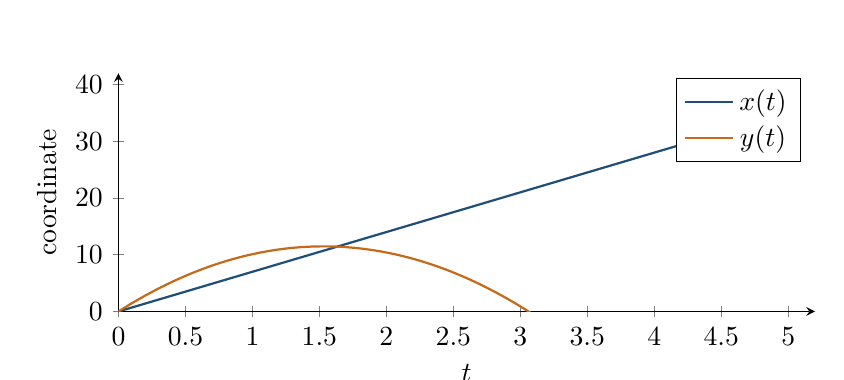
\begin{tikzpicture}
\begin{axis}[
width=0.86\textwidth,height=0.38\textwidth,
axis lines=left,
xlabel={$t$},ylabel={coordinate},
xmin=0,xmax=5.2,ymin=0,ymax=42,
legend style={at={(0.98,0.98)},anchor=north east},
]
\addplot[DeepBlue, thick, domain=0:5, samples=100] {7*x};
\addlegendentry{$x(t)$}
\addplot[WarmOrange, thick, domain=0:5, samples=100] {15*x-4.9*x*x};
\addlegendentry{$y(t)$}
\end{axis}
\end{tikzpicture}
\end{center}

The graph above is not the trajectory in space. It shows coordinates as functions of time. A common mistake is to confuse a graph of $y$ versus $t$ with the spatial path $y$ versus $x$. The vertical motion as a function of time is a parabola; the spatial path is also a parabola in this simple model, but for a different mathematical reason: time can be eliminated between the two component equations.

\begin{warningbox}{Do not confuse graphs}
A graph of $y(t)$ shows height versus time. A graph of $y(x)$ shows the shape of the path in space. They may look similar in projectile motion, but they answer different questions.
\end{warningbox}

\section{Eliminating time: the trajectory as a parabola}

Sometimes we do not ask where the projectile is at a particular time. Instead, we ask what curve it follows in the plane. Then we want $y$ directly as a function of $x$.

Assume for simplicity that $x_0=0$. From
\[
x(t)=v_0\cos\theta\,t
\]
we solve for $t$:
\[
t=\frac{x}{v_0\cos\theta}.
\]
This step is valid if $v_0\cos\theta\ne0$, meaning the projectile has nonzero horizontal velocity.

Substitute this time into the vertical equation:
\begin{align*}
y(x)&=y_0+v_0\sin\theta\left(\frac{x}{v_0\cos\theta}\right)-\frac12g\left(\frac{x}{v_0\cos\theta}\right)^2 \\
&=y_0+x\tan\theta-\frac{g}{2v_0^2\cos^2\theta}x^2.
\end{align*}

Thus
\[
\boxed{y(x)=y_0+x\tan\theta-\frac{g}{2v_0^2\cos^2\theta}x^2.}
\]

This is a quadratic function of $x$. Its graph is a parabola opening downward. The coefficient of $x^2$ is negative because gravity bends the trajectory downward.

\subsection{What the algebra means physically}

The term $x\tan\theta$ is what the height would be if the projectile continued in a straight line with its initial direction. The term
\[
-\frac{g}{2v_0^2\cos^2\theta}x^2
\]
is the downward correction caused by gravity. The farther the projectile travels horizontally, the more time gravity has had to act, and the downward correction grows like the square of time. Since time is proportional to $x$ in the horizontal motion, the correction becomes proportional to $x^2$.

\begin{principlebox}{Why a parabola appears}
The path is parabolic because horizontal motion is linear in time while vertical motion contains a quadratic term in time. Eliminating time transfers that quadratic dependence into the spatial curve $y(x)$.
\end{principlebox}

\newpage

\section{Landing on the ground: an equation of condition}

Now suppose the projectile is launched from ground level and lands on the same ground level. We set $y_0=0$. The vertical coordinate is
\[
y(t)=v_0\sin\theta\,t-\frac12gt^2.
\]
Landing on the ground means
\[
y(t)=0.
\]
Therefore
\[
v_0\sin\theta\,t-\frac12gt^2=0.
\]
Factor out $t$:
\[
t\left(v_0\sin\theta-\frac12gt\right)=0.
\]
So there are two solutions:
\[
t=0
\]
and
\[
t=\frac{2v_0\sin\theta}{g}.
\]

The first solution is the launch moment. It is not a mistake. The projectile is on the ground at the instant it is launched. The second solution is the landing time.

Thus the time of flight is
\[
\boxed{\tflight=\frac{2v_0\sin\theta}{g}.}
\]

\begin{methodbox}{Physical interpretation of the two roots}
A quadratic equation may produce several mathematical solutions. Physics tells us which solution represents which event. Here $t=0$ means launch; the positive nonzero root means landing.
\end{methodbox}

If $\theta=0$, then $\sin\theta=0$ and the formula gives $\tflight=0$ in the same-height idealization. That means a projectile fired perfectly horizontally from ground level would immediately be at ground level. In reality the object has size and the ground interaction matters. This shows that formulas must always be read together with the assumptions of the model.

\section{Range as the second intersection with the ground}

The horizontal position is
\[
x(t)=v_0\cos\theta\,t.
\]
At the landing time,
\[
R=x(\tflight).
\]
Substitute the flight time:
\begin{align*}
R&=v_0\cos\theta\left(\frac{2v_0\sin\theta}{g}\right) \\
&=\frac{2v_0^2\sin\theta\cos\theta}{g}.
\end{align*}
Using the identity
\[
\sin(2\theta)=2\sin\theta\cos\theta,
\]
we obtain
\[
\boxed{R=\frac{v_0^2\sin(2\theta)}{g}.}
\]

This is the famous range formula for launch and landing at the same height. But in this lecture we should not present it as a magic formula. It is the result of three ideas:
\begin{enumerate}
    \item vertical motion determines how long the projectile stays in the air;
    \item horizontal motion determines how far it moves during that time;
    \item same-height landing means solve $y(t)=0$ and choose the second root.
\end{enumerate}

\subsection{Range from the spatial parabola}

We can also find the range using the trajectory equation. With $y_0=0$,
\[
y(x)=x\tan\theta-\frac{g}{2v_0^2\cos^2\theta}x^2.
\]
Landing on the ground means $y(x)=0$:
\[
x\tan\theta-\frac{g}{2v_0^2\cos^2\theta}x^2=0.
\]
Factor:
\[
x\left(\tan\theta-\frac{g}{2v_0^2\cos^2\theta}x\right)=0.
\]
The two roots are
\[
x=0
\]
and
\[
x=\frac{2v_0^2\cos^2\theta\tan\theta}{g}.
\]
Since $\tan\theta=\dfrac{\sin\theta}{\cos\theta}$, the second root becomes
\[
x=\frac{2v_0^2\sin\theta\cos\theta}{g}=\frac{v_0^2\sin(2\theta)}{g}.
\]
So the same range is obtained.

\begin{principlebox}{Two mathematical routes, one physical event}
The range can be found from $y(t)=0$ and then $x(t)$, or directly from $y(x)=0$. The first route emphasizes time of flight; the second emphasizes intersections of the trajectory with the ground.
\end{principlebox}

This is an excellent classroom moment. The point is not to memorize two derivations. The point is to see that a physical event can be represented in different mathematical languages.

\newpage

\section{Maximum height: the top is a mathematical maximum}

The highest point is the maximum of the vertical coordinate. There are two natural ways to find it.

\subsection{Method 1: vertical velocity becomes zero}

The vertical velocity is
\[
v_y(t)=v_0\sin\theta-gt.
\]
At the top, the projectile stops moving upward for an instant before moving downward. Therefore
\[
v_y(t)=0.
\]
So
\[
v_0\sin\theta-gt=0,
\]
and
\[
\boxed{t_{\mathrm{up}}=\frac{v_0\sin\theta}{g}.}
\]
This is the time to reach the maximum height.

Substitute this time into $y(t)$, assuming $y_0=0$:
\begin{align*}
H_{\max}&=v_0\sin\theta\left(\frac{v_0\sin\theta}{g}\right)-\frac12g\left(\frac{v_0\sin\theta}{g}\right)^2 \\
&=\frac{v_0^2\sin^2\theta}{g}-\frac12\frac{v_0^2\sin^2\theta}{g} \\
&=\frac{v_0^2\sin^2\theta}{2g}.
\end{align*}
Thus
\[
\boxed{H_{\max}=\frac{v_0^2\sin^2\theta}{2g}.}
\]

\subsection{Method 2: maximize the height function}

The height is a quadratic function of time:
\[
y(t)=v_0\sin\theta\,t-\frac12gt^2.
\]
The derivative is
\[
\dv{y}{t}=v_0\sin\theta-gt.
\]
Set the derivative equal to zero:
\[
\dv{y}{t}=0.
\]
This gives the same condition as $v_y=0$, because velocity is the derivative of position.

\subsection{Why the answer makes sense}

The maximum height depends on the square of the vertical component of the initial velocity:
\[
H_{\max}=\frac{v_{0y}^2}{2g}.
\]
The horizontal component does not directly affect the maximum height. It affects how far sideways the projectile moves while it rises, but not how high it rises in the ideal model.

If $\theta=0$, then the vertical component is zero and $H_{\max}=0$. If $\theta=90^\circ$, all the speed is vertical and the height is maximal for the given speed. This interpretation checks the formula.

\begin{methodbox}{A useful habit}
After deriving a formula, test it in extreme cases. What happens at $\theta=0$? What happens at $\theta=90^\circ$? What happens if $v_0$ doubles? This is not extra work. It is part of understanding the result.
\end{methodbox}

\section{Time up, time down, and symmetry}

For launch and landing at the same height, the time to reach the top is
\[
t_{\mathrm{up}}=\frac{v_0\sin\theta}{g}.
\]
The total time of flight is
\[
t_{\mathrm{flight}}=\frac{2v_0\sin\theta}{g}.
\]
Therefore
\[
t_{\mathrm{flight}}=2t_{\mathrm{up}}.
\]
The time upward equals the time downward.

This symmetry is not a universal truth about all projectile motion. It depends on same launch and landing height and no air resistance. If the projectile lands below the launch height, the falling part takes longer. If it lands above the launch height, the total time can be shorter.

\subsection{Velocity symmetry}

At launch, the vertical velocity is $v_0\sin\theta$. At landing on the same level, the vertical velocity is
\[
v_y(t_{\mathrm{flight}})=v_0\sin\theta-g\left(\frac{2v_0\sin\theta}{g}\right)=-v_0\sin\theta.
\]
So the vertical velocity has the same magnitude and opposite sign. The horizontal velocity remains $v_0\cos\theta$. Therefore the speed at landing equals the speed at launch in this ideal model.

This is another example of a formula expressing a physical idea. With no air resistance and same height, mechanical energy is conserved; the speed returns to the same magnitude.

\section{Launch from a height: when the symmetry disappears}

Now suppose the projectile is launched from height $y_0>0$ and lands on the ground $y=0$. The vertical coordinate is
\[
y(t)=y_0+v_0\sin\theta\,t-\frac12gt^2.
\]
Landing means
\[
y_0+v_0\sin\theta\,t-\frac12gt^2=0.
\]
This is a quadratic equation. To make the leading coefficient positive, multiply by $-1$:
\[
\frac12gt^2-v_0\sin\theta\,t-y_0=0.
\]
Using the quadratic formula,
\[
t=\frac{v_0\sin\theta\pm\sqrt{v_0^2\sin^2\theta+2gy_0}}{g}.
\]
The physically relevant landing time is the positive root:
\[
\boxed{t_{\mathrm{flight}}=\frac{v_0\sin\theta+\sqrt{v_0^2\sin^2\theta+2gy_0}}{g}.}
\]
The negative root corresponds to a time before launch at which the mathematical parabola would have crossed the ground if extended backward. It is mathematically valid but not the future landing event.

The horizontal range is then
\[
\boxed{R=v_0\cos\theta\,t_{\mathrm{flight}}.}
\]
That is,
\[
R=\frac{v_0\cos\theta}{g}\left(v_0\sin\theta+\sqrt{v_0^2\sin^2\theta+2gy_0}\right).
\]

\begin{warningbox}{Same symbol, different formula}
The simple formula $R=v_0^2\sin(2\theta)/g$ is not the general range formula. It assumes launch and landing at the same height. If the height changes, the time of flight changes first, and the range changes with it.
\end{warningbox}

\section{Projectile launched horizontally from a height}

A useful special case is horizontal launch. Then $\theta=0$ and $v_{0y}=0$. The equations become
\[
x(t)=v_0t,
\qquad
 y(t)=y_0-\frac12gt^2.
\]
Landing means
\[
y_0-\frac12gt^2=0.
\]
Thus
\[
t=\sqrt{\frac{2y_0}{g}}.
\]
The range is
\[
R=v_0\sqrt{\frac{2y_0}{g}}.
\]

This case is conceptually important because it shows clearly that horizontal and vertical motions are linked by the same time. The object does not ``finish horizontal motion'' and then ``start falling''. It moves horizontally while falling.

\subsection{Physical reading}

The time of flight depends only on the height $y_0$ and gravity $g$, not on the horizontal speed $v_0$. The horizontal speed determines how far the object travels during that fall time. If the table is higher, the object has more time to move horizontally. If the initial horizontal speed is larger, it covers more horizontal distance in the same fall time.

This result often surprises students because everyday language separates sideways motion and falling. The mathematics forces a clearer statement: both components evolve during the same time interval.

\newpage

\section{Hitting a target: equations become constraints}

Suppose a target is located at $(X,Y)$ relative to the launch point. We ask whether a projectile launched with speed $v_0$ and angle $\theta$ can hit it.

Using the trajectory equation with $y_0=0$,
\[
y(x)=x\tan\theta-\frac{g}{2v_0^2\cos^2\theta}x^2.
\]
To hit the target, the point $(X,Y)$ must lie on the trajectory. Therefore
\[
Y=X\tan\theta-\frac{gX^2}{2v_0^2\cos^2\theta}.
\]
This is not a final formula to memorize. It is the mathematical translation of the sentence:

\emph{At horizontal position $X$, the projectile's height must be $Y$.}

Depending on what is known and what is unknown, this same equation can be used in different ways.

\subsection{Known angle, find required speed}

If $X$, $Y$, and $\theta$ are known, solve for $v_0^2$:
\[
Y=X\tan\theta-\frac{gX^2}{2v_0^2\cos^2\theta}.
\]
Move the gravity term:
\[
X\tan\theta-Y=\frac{gX^2}{2v_0^2\cos^2\theta}.
\]
Thus
\[
v_0^2=\frac{gX^2}{2\cos^2\theta\,(X\tan\theta-Y)}.
\]
So
\[
\boxed{v_0=\sqrt{\frac{gX^2}{2\cos^2\theta\,(X\tan\theta-Y)}}.}
\]
This only makes physical sense if $X\tan\theta-Y>0$. That condition says the straight line in the initial direction must pass above the target; gravity then bends the projectile down to reach it.

\subsection{Known speed, find possible angles}

If $X$, $Y$, and $v_0$ are known, the unknown is $\theta$. The equation is more complicated. It may have zero, one, or two solutions. Physically, two solutions correspond to a low trajectory and a high trajectory.

This is an important lesson: the same target can often be hit in more than one way. The mathematics does not merely compute a number; it describes the structure of possibilities.

\begin{principlebox}{Equations can express possibility}
When we write the target condition, we are not only calculating. We are asking whether the target lies on some possible trajectory. A solution means possible; no solution means impossible under the chosen assumptions.
\end{principlebox}

\section{Passing through a window: inequalities and intervals}

Now suppose the projectile must pass through a vertical window located at horizontal position $X$. The window extends from height $Y_1$ to height $Y_2$. The condition is not an equality, but an inequality:
\[
Y_1\le y(X)\le Y_2.
\]
Using the trajectory equation,
\[
Y_1\le X\tan\theta-\frac{gX^2}{2v_0^2\cos^2\theta}\le Y_2.
\]
This inequality says that the projectile's height at the window's horizontal position must lie between the bottom and top of the window.

If $v_0$ is fixed and $\theta$ can vary, this inequality describes a range of allowed angles. If $\theta$ is fixed and $v_0$ can vary, it describes a range of allowed speeds. If both can vary, it describes a region in parameter space.

\subsection{Why this matters pedagogically}

Students often expect physics problems to end with a single number. But real physical questions often ask for admissible ranges: safe speeds, possible angles, acceptable tolerances, times during which a condition holds. Inequalities are the mathematical language for such questions.

\begin{examplebox}{Mini-example: height at a gate}
A projectile is launched from ground level with $v_0=20\,\mathrm{m/s}$ at $45^\circ$. A gate is at $X=20\,\mathrm{m}$. Ignoring air resistance, estimate the height at the gate.

We use
\[
y(X)=X\tan\theta-\frac{gX^2}{2v_0^2\cos^2\theta}.
\]
For $\theta=45^\circ$, $\tan\theta=1$ and $\cos^2\theta=1/2$. Thus
\[
y(20)=20-\frac{9.81\cdot 20^2}{2\cdot 20^2\cdot 1/2}
=20-9.81\approx 10.19\,\mathrm{m}.
\]
The result is not just a number. It says the projectile is still high above the ground at $20\,\mathrm{m}$ horizontally.
\end{examplebox}

\section{Maximum range for a fixed launch speed}

For launch and landing at the same height, the range is
\[
R(\theta)=\frac{v_0^2\sin(2\theta)}{g}.
\]
Now the angle $\theta$ becomes the variable. The speed $v_0$ and gravity $g$ are fixed parameters. The physical question

\emph{Which angle gives the largest range?}

becomes the mathematical question
\[
\text{maximize } R(\theta).
\]
Since $v_0^2/g$ is constant, we maximize $\sin(2\theta)$. The maximum value of sine is $1$, attained when
\[
2\theta=90^\circ.
\]
Therefore
\[
\boxed{\theta=45^\circ}
\]
and
\[
\boxed{R_{\max}=\frac{v_0^2}{g}.}
\]

\subsection{Derivative method}

If we use calculus, differentiate:
\[
R'(\theta)=\frac{v_0^2}{g}\cdot 2\cos(2\theta).
\]
Set the derivative equal to zero:
\[
\cos(2\theta)=0.
\]
For launch angles between $0^\circ$ and $90^\circ$, this gives $2\theta=90^\circ$, so $\theta=45^\circ$.

\subsection{Physical interpretation}

At small angles, the projectile has large horizontal velocity but little time in the air. At large angles, it stays in the air longer but has small horizontal velocity. The best range balances these two effects. The angle $45^\circ$ is not magic; it is the balance point in the same-height, no-air-resistance model.

\begin{warningbox}{The $45^\circ$ result is conditional}
The $45^\circ$ result assumes launch and landing at the same height and no air resistance. If the landing point is lower, the optimal angle is usually less than $45^\circ$. If air resistance matters, the optimal angle also changes.
\end{warningbox}

\section{Complementary angles and the same range}

The range formula
\[
R(\theta)=\frac{v_0^2\sin(2\theta)}{g}
\]
shows that two different angles can give the same range. Since
\[
\sin(2\theta)=\sin(180^\circ-2\theta),
\]
the angles $\theta$ and $90^\circ-\theta$ give the same range.

For example, $30^\circ$ and $60^\circ$ have the same ideal range because
\[
\sin(60^\circ)=\sin(120^\circ).
\]
But the trajectories are not the same. The $30^\circ$ trajectory is lower and faster horizontally. The $60^\circ$ trajectory is higher and stays in the air longer.

\subsection{Same range does not mean same motion}

This is another place where formulas must be interpreted carefully. The equality of ranges does not imply equality of flight times, maximum heights, or velocities at intermediate points. It only says that the final horizontal displacement is the same.

\begin{examplebox}{Comparing $30^\circ$ and $60^\circ$}
For the same $v_0$:
\[
R_{30}=R_{60}.
\]
But
\[
H_{\max,60}=\frac{v_0^2\sin^2 60^\circ}{2g}
=3\frac{v_0^2}{8g},
\]
while
\[
H_{\max,30}=\frac{v_0^2\sin^2 30^\circ}{2g}
=\frac{v_0^2}{8g}.
\]
Thus the $60^\circ$ shot reaches three times the maximum height of the $30^\circ$ shot, even though their ranges are equal.
\end{examplebox}

\newpage

\section{The same model seen through energy}

Although the main derivations used kinematics, maximum height can also be found by energy. At launch, the vertical part of kinetic energy associated with upward motion is
\[
\frac12m(v_0\sin\theta)^2.
\]
At the highest point, the vertical component of velocity is zero, so this part has been converted into gravitational potential energy:
\[
mgH_{\max}=\frac12m(v_0\sin\theta)^2.
\]
Cancel $m$:
\[
H_{\max}=\frac{v_0^2\sin^2\theta}{2g}.
\]
This is the same result as before.

\subsection{Why multiple derivations are useful}

A second derivation is not merely a check. It shows that different physical principles can lead to the same conclusion. Kinematics describes how motion changes in time. Energy describes a transformation between kinetic and potential forms. Both are valid inside the same ideal model.

\begin{principlebox}{Multiple descriptions deepen understanding}
When two methods give the same result, we should not only celebrate the answer. We should ask what each method reveals. Kinematics reveals time structure; energy reveals conversion and conservation.
\end{principlebox}

Energy does not directly give the range, because range depends on time and horizontal motion. Kinematics is more natural for that. This illustrates a strategic point: different mathematical tools are suited to different questions.

\section{Dimensional analysis: reading units as meaning}

Units are not decoration. They are part of the meaning of quantities. A correct physical equation must be dimensionally consistent.

Consider the range formula:
\[
R=\frac{v_0^2\sin(2\theta)}{g}.
\]
The sine factor is dimensionless. The unit of $v_0^2$ is
\[
\left(\frac{\mathrm{m}}{\mathrm{s}}\right)^2=\frac{\mathrm{m^2}}{\mathrm{s^2}}.
\]
The unit of $g$ is
\[
\frac{\mathrm{m}}{\mathrm{s^2}}.
\]
Therefore
\[
\frac{v_0^2}{g}
\quad\text{has unit}\quad
\frac{\mathrm{m^2/s^2}}{\mathrm{m/s^2}}=\mathrm{m}.
\]
So the right-hand side has units of length, as a range should.

\subsection{Dimensional interpretation}

The factor $v_0^2/g$ is a natural length scale for projectile motion. A larger initial speed increases range quadratically; stronger gravity decreases range. The angle determines what fraction of that natural length scale is achieved.

\begin{methodbox}{Unit check}
Before trusting a result, check its units. A formula for time should have units of seconds. A formula for height or range should have units of meters. If the units fail, the expression cannot be physically correct.
\end{methodbox}

\section{Graphs as arguments, not pictures}

A graph in physics is not merely an illustration. It can be an argument. For projectile motion, the graph of $y(t)$ is a downward-opening parabola. The roots of this graph represent times when the projectile is at ground level. The vertex represents maximum height.

\begin{center}
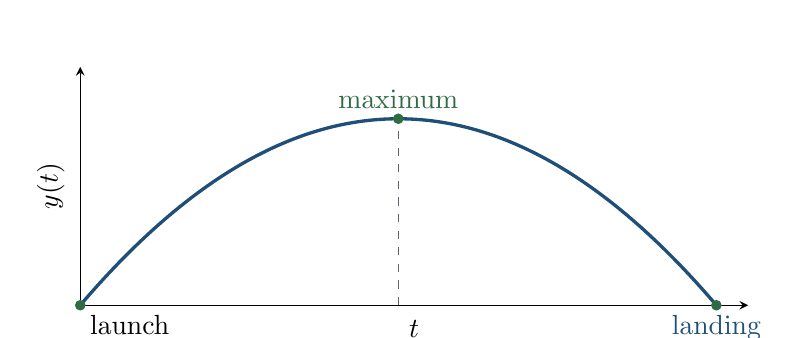
\begin{tikzpicture}
\begin{axis}[
width=0.83\textwidth,height=0.38\textwidth,
axis lines=left,
xlabel={$t$},ylabel={$y(t)$},
xmin=0,xmax=6.3,ymin=0,ymax=23,
xtick=\empty,ytick=\empty,
clip=false]
\addplot[DeepBlue, very thick, domain=0:6, samples=160] {12*x-2*x*x};
\addplot[only marks, mark=*, mark size=1.7pt, DeepGreen] coordinates {(0,0) (3,18) (6,0)};
\node[anchor=south, DeepGreen] at (axis cs:3,18) {maximum};
\node[anchor=north, DeepBlue] at (axis cs:6,0) {landing};
\node[anchor=north west] at (axis cs:0,0) {launch};
\draw[dashed, GraphGrey] (axis cs:3,0) -- (axis cs:3,18);
\end{axis}
\end{tikzpicture}
\end{center}

Reading this graph mathematically:
\begin{itemize}
    \item roots answer ``when is the projectile at ground level?''
    \item the vertex answers ``when and where is the height maximal?''
    \item the slope answers ``what is the vertical velocity?''
    \item concavity answers ``what is the sign of vertical acceleration?''
\end{itemize}

A single graph therefore contains many pieces of physical information. The formulas and graphs are not separate worlds. They are different representations of the same model.

\section{A fully worked example: one launch, many questions}

Let a projectile be launched from ground level with initial speed
\[
v_0=20\,\mathrm{m/s}
\]
at angle
\[
\theta=30^\circ.
\]
Use $g=9.81\,\mathrm{m/s^2}$.

\subsection{Step 1: components}

The horizontal component is
\[
v_{0x}=v_0\cos30^\circ=20\cdot\frac{\sqrt3}{2}=10\sqrt3\approx17.32\,\mathrm{m/s}.
\]
The vertical component is
\[
v_{0y}=v_0\sin30^\circ=20\cdot\frac12=10\,\mathrm{m/s}.
\]

\subsection{Step 2: equations of motion}

With launch from ground level,
\[
x(t)=17.32t,
\]
\[
y(t)=10t-4.905t^2.
\]
These equations are the model for this particular launch.

\subsection{Step 3: time of flight}

Landing means $y(t)=0$:
\[
10t-4.905t^2=0.
\]
Factor:
\[
t(10-4.905t)=0.
\]
The nonzero root is
\[
t=\frac{10}{4.905}\approx2.04\,\mathrm{s}.
\]
This is the time in the air.

\subsection{Step 4: range}

The range is horizontal position at landing:
\[
R=x(2.04)\approx17.32\cdot2.04\approx35.3\,\mathrm{m}.
\]

\subsection{Step 5: maximum height}

The time to the top is
\[
t_{\mathrm{up}}=\frac{v_{0y}}{g}=\frac{10}{9.81}\approx1.02\,\mathrm{s}.
\]
The maximum height is
\[
H_{\max}=\frac{v_{0y}^2}{2g}=\frac{100}{19.62}\approx5.10\,\mathrm{m}.
\]

\subsection{Step 6: interpretation}

The object moves fast horizontally, but its vertical component is only $10\,\mathrm{m/s}$. It reaches a height of about five meters, stays in the air for about two seconds, and lands about thirty-five meters away. These numbers tell a coherent story. The flight time is twice the time to the top because launch and landing heights are the same.

\begin{principlebox}{What this example demonstrates}
We did not begin by selecting disconnected formulas. We built one model, asked several questions, and extracted several answers from the same mathematical structure.
\end{principlebox}

\section{A target example: translating a sentence into an equation}

A projectile is launched from ground level with speed $v_0=25\,\mathrm{m/s}$ at angle $40^\circ$. Will it pass through a point located $30\,\mathrm{m}$ away horizontally and $8\,\mathrm{m}$ above the ground?

\subsection{Physical sentence}

At horizontal coordinate $x=30\,\mathrm{m}$, the vertical coordinate must be $y=8\,\mathrm{m}$.

\subsection{Mathematical translation}

Use
\[
y(x)=x\tan\theta-\frac{gx^2}{2v_0^2\cos^2\theta}.
\]
Evaluate at $x=30$:
\[
y(30)=30\tan40^\circ-\frac{9.81\cdot30^2}{2\cdot25^2\cos^240^\circ}.
\]
Using approximate values $\tan40^\circ\approx0.8391$ and $\cos40^\circ\approx0.7660$,
\[
y(30)\approx25.17-\frac{8829}{2\cdot625\cdot0.5868}.
\]
The denominator is about $733.5$, so
\[
y(30)\approx25.17-12.04=13.13\,\mathrm{m}.
\]

\subsection{Interpretation}

At $x=30\,\mathrm{m}$ the projectile is approximately $13.1\,\mathrm{m}$ above the ground, not $8\,\mathrm{m}$. Therefore it does not pass through the target point. It passes above it.

This is a good example because the answer is not obtained by a special ``target formula''. We simply evaluate the trajectory at a given horizontal position.

\section{An inverse example: finding a speed from a desired hit}

Suppose a projectile must pass through a target at $X=20\,\mathrm{m}$ and $Y=5\,\mathrm{m}$. The launch angle is fixed at $45^\circ$. What initial speed is required?

The target condition is
\[
Y=X\tan\theta-\frac{gX^2}{2v_0^2\cos^2\theta}.
\]
For $\theta=45^\circ$,
\[
\tan45^\circ=1,
\qquad
\cos^245^\circ=\frac12.
\]
So
\[
5=20-\frac{g\cdot20^2}{2v_0^2\cdot1/2}.
\]
The denominator simplifies:
\[
2v_0^2\cdot\frac12=v_0^2.
\]
Thus
\[
5=20-\frac{400g}{v_0^2}.
\]
Move terms:
\[
15=\frac{400g}{v_0^2}.
\]
Therefore
\[
v_0^2=\frac{400g}{15}.
\]
With $g=9.81$,
\[
v_0^2\approx261.6,
\qquad
v_0\approx16.2\,\mathrm{m/s}.
\]

\subsection{What changed compared with the previous example?}

Previously the speed and angle were known, and the target condition was used to test whether the projectile passes through a point. Now the angle and target are known, and the same condition is used to solve for speed. The equation did not change; the role of the unknown changed.

\begin{methodbox}{Role of the unknown}
A formula does not know what it is ``for''. We decide which symbol is unknown based on the physical question. The same relation can be used to find time, distance, speed, angle, or feasibility.
\end{methodbox}

\newpage

\section{What changes when assumptions change?}

The projectile equations are not eternal truths independent of assumptions. They are true inside a model. If the model changes, the equations change.

\subsection{Air resistance}

If air resistance is included, there is a force opposite to the velocity. Then horizontal acceleration is no longer zero. The horizontal velocity decreases, the trajectory is not exactly parabolic, and the range is smaller than the no-resistance prediction.

This does not make the ideal model useless. It means the ideal model has a domain of usefulness. For slow, dense objects over short distances, it may be a good approximation. For a feather, a badminton shuttlecock, or a long-range projectile, it may be poor.

\subsection{Changing gravity}

If the motion covers very large distances or heights, the gravitational field may not be treated as constant. Then $g$ is not a fixed number, and the acceleration is not simply $(0,-g)$. The model becomes more complex.

\subsection{Large-scale Earth curvature}

For ordinary classroom projectile motion, the ground is treated as flat and the vertical direction is constant. For very long ranges, Earth curvature and rotation matter. Again, the simple formula is not wrong inside its assumptions; it is limited by them.

\begin{principlebox}{Models are conditional}
Every formula has a territory. Understanding a formula includes knowing where it applies and where it stops applying.
\end{principlebox}

\section{How to read a physics problem without hunting formulas}

When facing a problem, do not begin by searching memory for a final expression. Begin by reading the physical structure.

\subsection{Question type 1: position at a time}

If the problem asks ``where is the object after $t$ seconds?'', use the parametric equations:
\[
x(t),\qquad y(t).
\]
This is direct evaluation.

\subsection{Question type 2: time when something happens}

If the problem asks ``when does the object hit the ground?'', ``when does it reach height $h$?'', or ``when is it at a point?'', write a condition involving $t$, such as
\[
y(t)=0
\]
or
\[
y(t)=h.
\]
Then solve for time.

\subsection{Question type 3: maximum or minimum}

If the problem asks for a maximum height or maximum range, identify the function being optimized:
\[
y(t),\quad y(x),\quad R(\theta),\quad \text{etc.}
\]
Then use vertex properties, derivatives, or known bounds such as $\sin(2\theta)\le1$.

\subsection{Question type 4: hitting or passing through}

If the problem asks whether the projectile hits a point or passes through a region, write a geometric condition:
\[
y(X)=Y
\]
for a point, or
\[
Y_1\le y(X)\le Y_2
\]
for a vertical interval.

\subsection{Question type 5: dependence on parameters}

If the problem asks how an answer changes when angle, speed, or height changes, treat the result as a function of that parameter. For example,
\[
R(\theta)=\frac{v_0^2\sin(2\theta)}{g}.
\]
Now the object of study is not the projectile's path alone, but the dependence of the range on launch angle.

\section{A compact map of projectile motion questions}

\begin{center}
\renewcommand{\arraystretch}{1.35}
\begin{tabular}{p{0.25\textwidth}p{0.33\textwidth}p{0.30\textwidth}}
\toprule
Physical question & Mathematical condition or object & Typical operation \\
\midrule
Where is it after time $t$? & $x(t), y(t)$ & evaluate functions \\
When does it land? & $y(t)=0$ & solve equation for $t$ \\
What is the range? & $x(t_{\mathrm{flight}})$ or $y(x)=0$ & solve and substitute \\
What is the maximum height? & $v_y(t)=0$ or $y'(t)=0$ & derivative / vertex \\
What angle gives max range? & $R(\theta)$ & maximize function \\
Does it hit a target? & $y(X)=Y$ & test or solve constraint \\
Does it pass through a window? & $Y_1\le y(X)\le Y_2$ & solve inequality \\
How does speed affect range? & $R(v_0)$ & analyze parameter dependence \\
\bottomrule
\end{tabular}
\end{center}

This table is not meant to replace understanding. It is meant to show how different physical questions correspond to different mathematical actions.

\newpage

\section{Common student mistakes and how to correct them}

\subsection{Mistake 1: using a formula outside its assumptions}

A student uses
\[
R=\frac{v_0^2\sin(2\theta)}{g}
\]
for a projectile launched from a cliff. The mistake is not algebraic. It is modelling: the formula assumes launch and landing at the same height.

Correction: return to
\[
y(t)=y_0+v_0\sin\theta\,t-\frac12gt^2
\]
and solve $y(t)=0$ with the actual $y_0$.

\subsection{Mistake 2: confusing $y(t)$ and $y(x)$}

A student sees a parabola and treats the time graph as the spatial path. Correction: ask what is on the horizontal axis. If the horizontal axis is $t$, the graph describes height over time. If it is $x$, the graph describes the shape of the path.

\subsection{Mistake 3: ignoring the physical meaning of roots}

When solving $y(t)=0$, a student obtains two roots and discards one without explanation. Correction: interpret each root. In same-height launch, $t=0$ is launch and the positive nonzero root is landing. In launch from height, a negative root may be a backward-time intersection.

\subsection{Mistake 4: treating signs as arbitrary}

A student writes $+\frac12gt^2$ instead of $-\frac12gt^2$ because ``gravity is positive''. Correction: define the coordinate system first. If upward is positive, the vertical acceleration is $-g$.

\subsection{Mistake 5: thinking that every question needs a new formula}

A student asks for the formula for passing through a window. Correction: there is no special formula. Use the trajectory equation and express the window as an inequality.

\section{Board plan for a 90-minute lecture}

This section is written as a practical lecture route. It can be followed directly on the board.

\subsection*{Part 1: Fifteen minutes - formulas as compressed statements}
\addcontentsline{toc}{subsection}{Part 1: Fifteen minutes - formulas as compressed statements}

Begin with three equations:
\[
F=ma,
\qquad
 y(t)=y_0+v_{0y}t-\frac12gt^2,
\qquad
 y(t)=0.
\]
Ask students: are these the same kind of thing? The point is to separate a law, a model equation, and a condition.

Then write the loop:
\[
\text{situation}\to\text{model}\to\text{mathematics}\to\text{interpretation}.
\]
Return to this loop throughout the lecture.

\subsection*{Part 2: Twenty minutes - building the model}
\addcontentsline{toc}{subsection}{Part 2: Twenty minutes - building the model}

Draw axes. Define assumptions. Write
\[
\vect a=(0,-g).
\]
Integrate to get velocity and position. Emphasize where initial conditions enter. Do not rush to range.

\subsection*{Part 3: Twenty minutes - extracting questions}
\addcontentsline{toc}{subsection}{Part 3: Twenty minutes - extracting questions}

Ask in sequence:
\begin{enumerate}
    \item When does it land? $y(t)=0$.
    \item How far does it go? $x(t_{\mathrm{flight}})$.
    \item How high does it go? $v_y(t)=0$.
    \item What curve does it follow? eliminate $t$.
\end{enumerate}
Show that these are different questions asked of the same model.

\subsection*{Part 4: Twenty minutes - changing the question}
\addcontentsline{toc}{subsection}{Part 4: Twenty minutes - changing the question}

Use a target or window example. Show that equality and inequality are physical conditions. Then show maximum range as an optimization problem in $\theta$.

\subsection*{Part 5: Fifteen minutes - summary and student practice}
\addcontentsline{toc}{subsection}{Part 5: Fifteen minutes - summary and student practice}

Give students a new physical sentence and ask them only to translate it mathematically. For example:
\begin{itemize}
    \item ``It reaches the top.'' $\rightarrow v_y(t)=0$.
    \item ``It lands on the ground.'' $\rightarrow y(t)=0$.
    \item ``It passes through a window.'' $\rightarrow Y_1\le y(X)\le Y_2$.
    \item ``It has maximum range.'' $\rightarrow$ maximize $R(\theta)$.
\end{itemize}
The aim is not speed of calculation, but correct translation.

\newpage

\section{Practice tasks focused on interpretation}

These tasks are designed to train translation, not long computation.

\subsection*{Task 1: identify the mathematical condition}
\addcontentsline{toc}{subsection}{Task 1: identify the mathematical condition}

A projectile is launched from ground level. Write the mathematical condition corresponding to each physical sentence.

\begin{enumerate}
    \item The projectile lands on the ground.
    \item The projectile reaches its highest point.
    \item The projectile passes through a point $(X,Y)$.
    \item The projectile passes through a vertical window at $x=X$ from height $Y_1$ to $Y_2$.
    \item The projectile has maximum range for fixed $v_0$.
\end{enumerate}

Expected translations:
\begin{enumerate}
    \item $y(t)=0$.
    \item $v_y(t)=0$ or $\dv{y}{t}=0$.
    \item $y(X)=Y$.
    \item $Y_1\le y(X)\le Y_2$.
    \item maximize $R(\theta)$.
\end{enumerate}

\subsection*{Task 2: same model, different questions}
\addcontentsline{toc}{subsection}{Task 2: same model, different questions}

For
\[
x(t)=12t,
\qquad
 y(t)=8t-4.9t^2,
\]
answer:
\begin{enumerate}
    \item What is the initial horizontal velocity?
    \item What is the initial vertical velocity?
    \item What is the vertical acceleration?
    \item When does the projectile land?
    \item When does it reach maximum height?
\end{enumerate}

Solution:
\begin{enumerate}
    \item $v_x=12\,\mathrm{m/s}$.
    \item $v_{0y}=8\,\mathrm{m/s}$.
    \item $a_y=-9.8\,\mathrm{m/s^2}$.
    \item Solve $8t-4.9t^2=0$, giving $t=0$ and $t=8/4.9\approx1.63\,\mathrm{s}$; landing is the second root.
    \item $v_y(t)=8-9.8t$, so $v_y=0$ gives $t=8/9.8\approx0.82\,\mathrm{s}$.
\end{enumerate}

\subsection*{Task 3: interpret a wrong formula choice}
\addcontentsline{toc}{subsection}{Task 3: interpret a wrong formula choice}

A student uses $R=v_0^2\sin(2\theta)/g$ for a projectile launched horizontally from a table of height $h$. Explain why this is wrong and what should be done instead.

Answer: the formula assumes launch and landing at the same height. A horizontal launch from a table has $y_0=h$ and $v_{0y}=0$. Use
\[
y(t)=h-\frac12gt^2
\]
to find the fall time, then use
\[
x(t)=v_0t
\]
to find the range.

\section{A short philosophical summary for students}

Physics uses mathematics because mathematics is a precise language for relations. A physical quantity rarely exists alone. Force relates to acceleration. Position relates to time. Velocity relates to change of position. Energy relates to height and speed. A formula is a compact way of writing such relations.

But compact writing is dangerous if we forget what has been compressed. The expression
\[
R=\frac{v_0^2\sin(2\theta)}{g}
\]
contains assumptions: no air resistance, constant gravity, launch and landing at the same height, fixed initial speed, angle measured from the horizontal. It also contains a story: vertical motion determines flight time, horizontal motion converts that time into distance, and trigonometry connects the components to the initial speed.

To understand physics is not to memorize the greatest number of formulas. It is to understand how formulas are born, what they mean, how they are used, and when they stop applying.

\begin{principlebox}{Final lecture sentence}
In physics, formulas are not magic keys. They are compressed meanings. The real skill is to unpack the meaning, use the mathematical structure, and pack the result back into a physical interpretation.
\end{principlebox}

\newpage

\appendix

\section{Algebra toolkit used in the notes}

\subsection{Solving a simple quadratic by factoring}

When we have
\[
at-bt^2=0,
\]
factor out $t$:
\[
t(a-bt)=0.
\]
Therefore
\[
t=0
\quad\text{or}\quad
 t=\frac{a}{b}.
\]
This is the structure of same-height landing:
\[
v_0\sin\theta\,t-\frac12gt^2=0.
\]

\subsection{Quadratic formula}

For
\[
At^2+Bt+C=0,
\]
the solutions are
\[
t=\frac{-B\pm\sqrt{B^2-4AC}}{2A}.
\]
In projectile motion from height $y_0$:
\[
\frac12gt^2-v_0\sin\theta\,t-y_0=0.
\]
Here
\[
A=\frac12g,
\quad
B=-v_0\sin\theta,
\quad
C=-y_0.
\]

\subsection{Vertex of a parabola}

For
\[
f(t)=at^2+bt+c,
\]
with $a<0$, the maximum occurs at
\[
t=-\frac{b}{2a}.
\]
For
\[
y(t)=-\frac12gt^2+v_0\sin\theta\,t+y_0,
\]
we have $a=-g/2$ and $b=v_0\sin\theta$, so
\[
t=\frac{v_0\sin\theta}{g}.
\]

\section{Trigonometry used in the notes}

The initial velocity vector has magnitude $v_0$ and angle $\theta$ above the horizontal. Its components are
\[
v_{0x}=v_0\cos\theta,
\qquad
v_{0y}=v_0\sin\theta.
\]
The tangent is
\[
\tan\theta=\frac{\sin\theta}{\cos\theta}.
\]
The double-angle identity is
\[
\sin(2\theta)=2\sin\theta\cos\theta.
\]
This identity is what transforms
\[
\frac{2v_0^2\sin\theta\cos\theta}{g}
\]
into
\[
\frac{v_0^2\sin(2\theta)}{g}.
\]

\section{Symbol glossary}

\begin{center}
\renewcommand{\arraystretch}{1.35}
\begin{tabular}{p{0.22\textwidth}p{0.68\textwidth}}
\toprule
Symbol & Meaning \\
\midrule
$t$ & time measured from launch \\
$x(t)$ & horizontal coordinate at time $t$ \\
$y(t)$ & vertical coordinate at time $t$ \\
$y(x)$ & trajectory height as a function of horizontal position \\
$v_0$ & initial speed \\
$\theta$ & launch angle above the horizontal \\
$v_{0x}$ & initial horizontal velocity component, $v_0\cos\theta$ \\
$v_{0y}$ & initial vertical velocity component, $v_0\sin\theta$ \\
$g$ & positive magnitude of gravitational acceleration near Earth's surface \\
$R$ & horizontal range \\
$H_{\max}$ & maximum height above launch level, when $y_0=0$ \\
$t_{\mathrm{up}}$ & time from launch to highest point \\
$t_{\mathrm{flight}}$ & total time in the air \\
$y_0$ & initial height above the chosen ground level \\
\bottomrule
\end{tabular}
\end{center}

\section{One-page summary of the core formulas}

This final page is intentionally compact. It should be used only after the modelling narrative is understood.

Assumptions: point-like projectile, no air resistance, constant downward gravitational acceleration, axes with $y$ upward.

\subsection*{Model}
\[
\vect a=(0,-g).
\]
\[
v_x(t)=v_0\cos\theta,
\qquad
v_y(t)=v_0\sin\theta-gt.
\]
\[
x(t)=x_0+v_0\cos\theta\,t,
\qquad
 y(t)=y_0+v_0\sin\theta\,t-\frac12gt^2.
\]

\subsection*{Trajectory}
For $x_0=0$:
\[
y(x)=y_0+x\tan\theta-\frac{g}{2v_0^2\cos^2\theta}x^2.
\]

\subsection*{Same launch and landing height}
If $y_0=0$ and landing occurs at $y=0$:
\[
t_{\mathrm{flight}}=\frac{2v_0\sin\theta}{g},
\]
\[
R=\frac{v_0^2\sin(2\theta)}{g},
\]
\[
t_{\mathrm{up}}=\frac{v_0\sin\theta}{g},
\]
\[
H_{\max}=\frac{v_0^2\sin^2\theta}{2g}.
\]

\begin{warningbox}{Use this page responsibly}
These formulas are not a replacement for the model. Each formula answers a particular question under particular assumptions. Always reconstruct the question before using the expression.
\end{warningbox}

\end{document}
